\documentclass[sheet=1, english]{dexercise}

\usepackage{graphicx}

\title{Computer Security}
\author{Basil Ugbomoiko\\Daniel Knaack}

\begin{document}

\task[Memory Addresses]

\begin{enumerate}
  \item
    Virtual memory is an abstraction that gives the illusion of large, uniform, private storage space.
    It maps a virtual address into a physical address by reading the page frame number from the page table.
    This enables isolation of processes.
    Each process has its own virtual address space and cannot access memory from another process without IPC.
    However, they still access the same physical memory albeit with different pages.
    In general, the virtual address space is larger than the physical address space.
    The physical memory is constrained by the actual size of the memory installed in the machine.


    The virtual memory is initialized by the operating system.
    It fills in a page table which defines how virtual addresses are translated.
    Physical memory is initialized not by the operating system but instead during boot-up by the system itself.
  \item
    \begin{enumerate}[\sffamily\color{maincolor}i.]
      \item
        The most-significant bits \texttt{vaddr[63:p]} determine the page frame
        number and the page offset is determined by the least-significant bits
        \texttt{vaddr[p-1:0]}.
      \item
        The bits that are used for the page offset won't be translated since
        they are used for indexing into the page itself.
    \end{enumerate}
  \item
    For x86\_64, you can tell by looking at the most-significant bits since only
    48 bits are used to get the physical memory address. If the most-significant
    bits are set to $1$, then this indicates that it is a kernel memory address.
    Otherwise, it indicates a user-level address.
  \item
    \begin{enumerate}[\sffamily\color{maincolor}i.]
      \item
        The virtual address space is $64 \cdot 1024 \cdot 2 = 131072$ bytes (128 KB) long.
      \item
        Since we have 32 frames, we need $5$ bits to encode the frame number.
        The pages are $1024 \cdot 2 = 2048$ bytes long, so we need $11$ bits to encode the offset.
        In total, we need $16$ bits to encode the physical address.
    \end{enumerate}
  \item
    A power-of-two page size makes it computationally easy to compute the page
    number and offset from the address. Computing the page number only requires
    a right shift and computing the offset requires a masking operation. For
    non-power-of-two page sizes, it would require an integer division and modulo
    operation to compute the page number and offset respectively.
  \item
    The two drawbacks are \emph{concurrency issues} and possible
    \emph{side-channel} through caching.

    If two programs have access to the same page with write access and one
    program reads the page and the other one writes to the page, then the first
    program could read corrupted data.

    If we eliminate write access, then there are still possible issues related
    to side channels. If one program reads the page, then it gets loaded into
    the cache. If another program reads the same page, then the page is already
    loaded in the cache, so the page access is faster. This opens the door to
    possible side-channel attacks.
  \item
    If the IOMMU is not activated or present, then the DMA can only work with
    physical addresses. Without the IOMMU, any I/O device with DMA has
    unrestricted access to any part of the physical memory. Thus, if any
    attacker has access to such an I/O device, we have no guarantee for security
    of our memory. A process cannot store any important data into memory since a
    device could read it using DMA.
  \item
    What happens on a context switch, depends on the specific CPU. For older
    CPUs, the TLB is simply flushed. However, this will impact performance since
    the TLB has to be filled again on each context switch. Thus, for newer CPUs,
    TLB entries are tagged with an additional process context identifier such
    that a cache hit only occurs when the PCID matches.
\end{enumerate}

\task[Page Fault Side Channel]

\begin{enumerate}
    \item
        \begin{enumerate}[\sffamily\color{maincolor}i.]
          \item
            \emph{Early Boot Phase}: This phase involves hardware initialization, such
            as the CPU, memory and devices. The bootloader (e.g GRUB or LILO in
            Linux Systems), is loaded and executed. The bootloader's role is to
            locate and load the kernel into memory and pass control to it.

            \emph{Kernel Initialization Phase}: Once control is passed to the kernel,
            it initializes its own data structures, sets up memory management,
            initializes devices, mounts the root filesystem, and starts the
            initial user-space process (init or systemd).

          \item
            The kernel typically resides in a protected memory region that is
            inaccessible to user-space applications. This protected region may
            be mapped to specific GFNs in the virtual machine's memory, ensuring
            that the kernel remains isolated and secure.

            Application processes operate within their own memory spaces,
            separate from the kernel. These processes have their own virtual
            addresses, which are translated to physical addresses by the memory
            management unit (MMU) based on the page tables set up for each
            process.

            \item Address Space Layout Randomization (ASLR): ASLR randomizes the memory addresses used by the kernel and user space processes, making it more difficult for attackers to predict the memory layout and locate specific kernel components.

            Kernel Address Space Isolation: Ensuring strict isolation between kernel space and user space memory can prevent unauthorized access and make it harder to exploit side channels to monitor kernel activities.

            Page Table Protection: Protecting the integrity of the page tables and preventing unauthorized modifications can help prevent side-channel attacks that rely on manipulating page table entries to trigger page faults.

 Hardware-Based Security Features: Utilizing hardware-based security features like Intel's SGX or AMD's SEV can provide additional layers of protection by encrypting sensitive data and ensuring secure execution environments for critical workloads.
        \end{enumerate}
    \item
    Figure~\ref{fig:runs} shows the location of the GFNs of both runs.
    We can clearly see that there are three main regions of page accesses.
    The first and third region are roughly the same for each run.
    However, the location second region is different.
    In the first run, the second region is located at a higher address than the second run.

    The second region starts at \texttt{0x1bc00} in the first run and \texttt{0x0b000} in the second.
    Thus, we conclude that the \texttt{.text} section is loaded at those respective addresses in each run.

    \begin{figure}
        \centering
        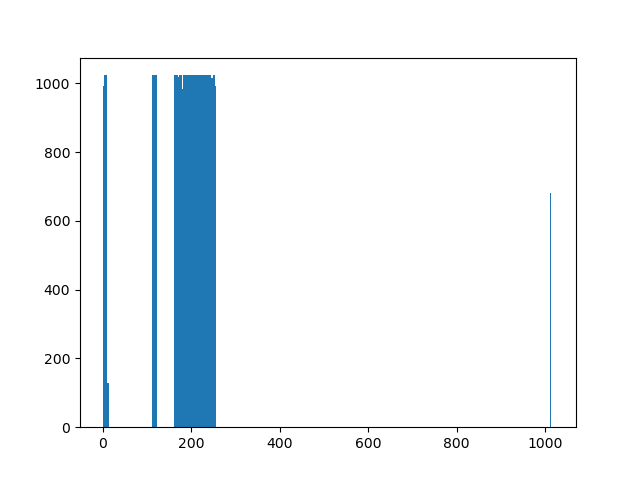
\includegraphics[width=0.4\textwidth]{run1.png}
        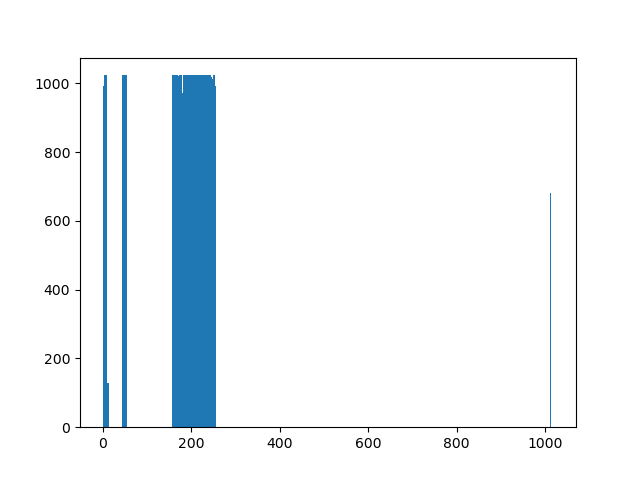
\includegraphics[width=0.4\textwidth]{run2.png}
        \caption{The number of times each GFN is accessed during the first and
        second run. Only the most-significant bits of each GFN are considered, i.e.
        two GFNs which have the same most-significant bits are counted as the same GFN.}
        \label{fig:runs}
    \end{figure}
\end{enumerate}

\end{document}
